\documentclass{standalone}
\begin{document}
	\subsection{Number of Clusters}
	
	The designed algorithm for the centroids estimation is the k-means clustering that requires a prior knowledge about the number of clusters to use. This is very important since a bad choice will badly affect the whole segmentation results. In order to chose the proper number of clusters, I've consider two different sources of information: the anatomical knowledge about the lung and the internal variability of the lung.
	
	From anatomical knowledge about the lung, we can derive 5 clusters, corresponding to: 
	
	\begin{itemize}
		\item Lung Parenchima; 
		
		\item  Edges;
		
		\item Vessel surrounding bronchial structures;
		
		
		\item Bronchi.
		
		\item  Ground Glass Opacities and Consolidation;
	\end{itemize}

	Notice that the background of the image is not considered as a cluster since it is removed from the segmentation for the reasons explained before.
	In order to verify that this number of clusters is the best one, I have considered the internal cluster variability.
	
	Clustering techniques try to group the data into different clusters  in order to maximize the difference between points in different clusters and to maximize the similarity within each cluster.  If the number of centroids is less then the clusters one, the similarity within each cluster is low. Increasing the number of centroids, will reduce reduce the internal variability till $0$ (if number of clusters is equal to the number of points). 
	This means that after a a certain point the diminishing of the internal variability is no more significant, since do not correspond to the good number of clusters but only to the increasing of their number.
	
	To found the correct number of clusters we are seek to for a number of clusters which still provides a small amount of internal variability. 
	
	To achieve this purpose, the clustering was repeated several times increasing the number of clusters and for each iteration the internal variability was measured by the sum of squares estimate error (SSE) : 
	\begin{equation}\label{eq:SumOfSquare}
		SSE = \sum (x_i - c_j)^2
	\end{equation}
	
	Once this task is completed, the results was printed in \figurename\,\ref{fig:ElbowCurve}. 
	
	\begin{figure}[h!]
		\centering
		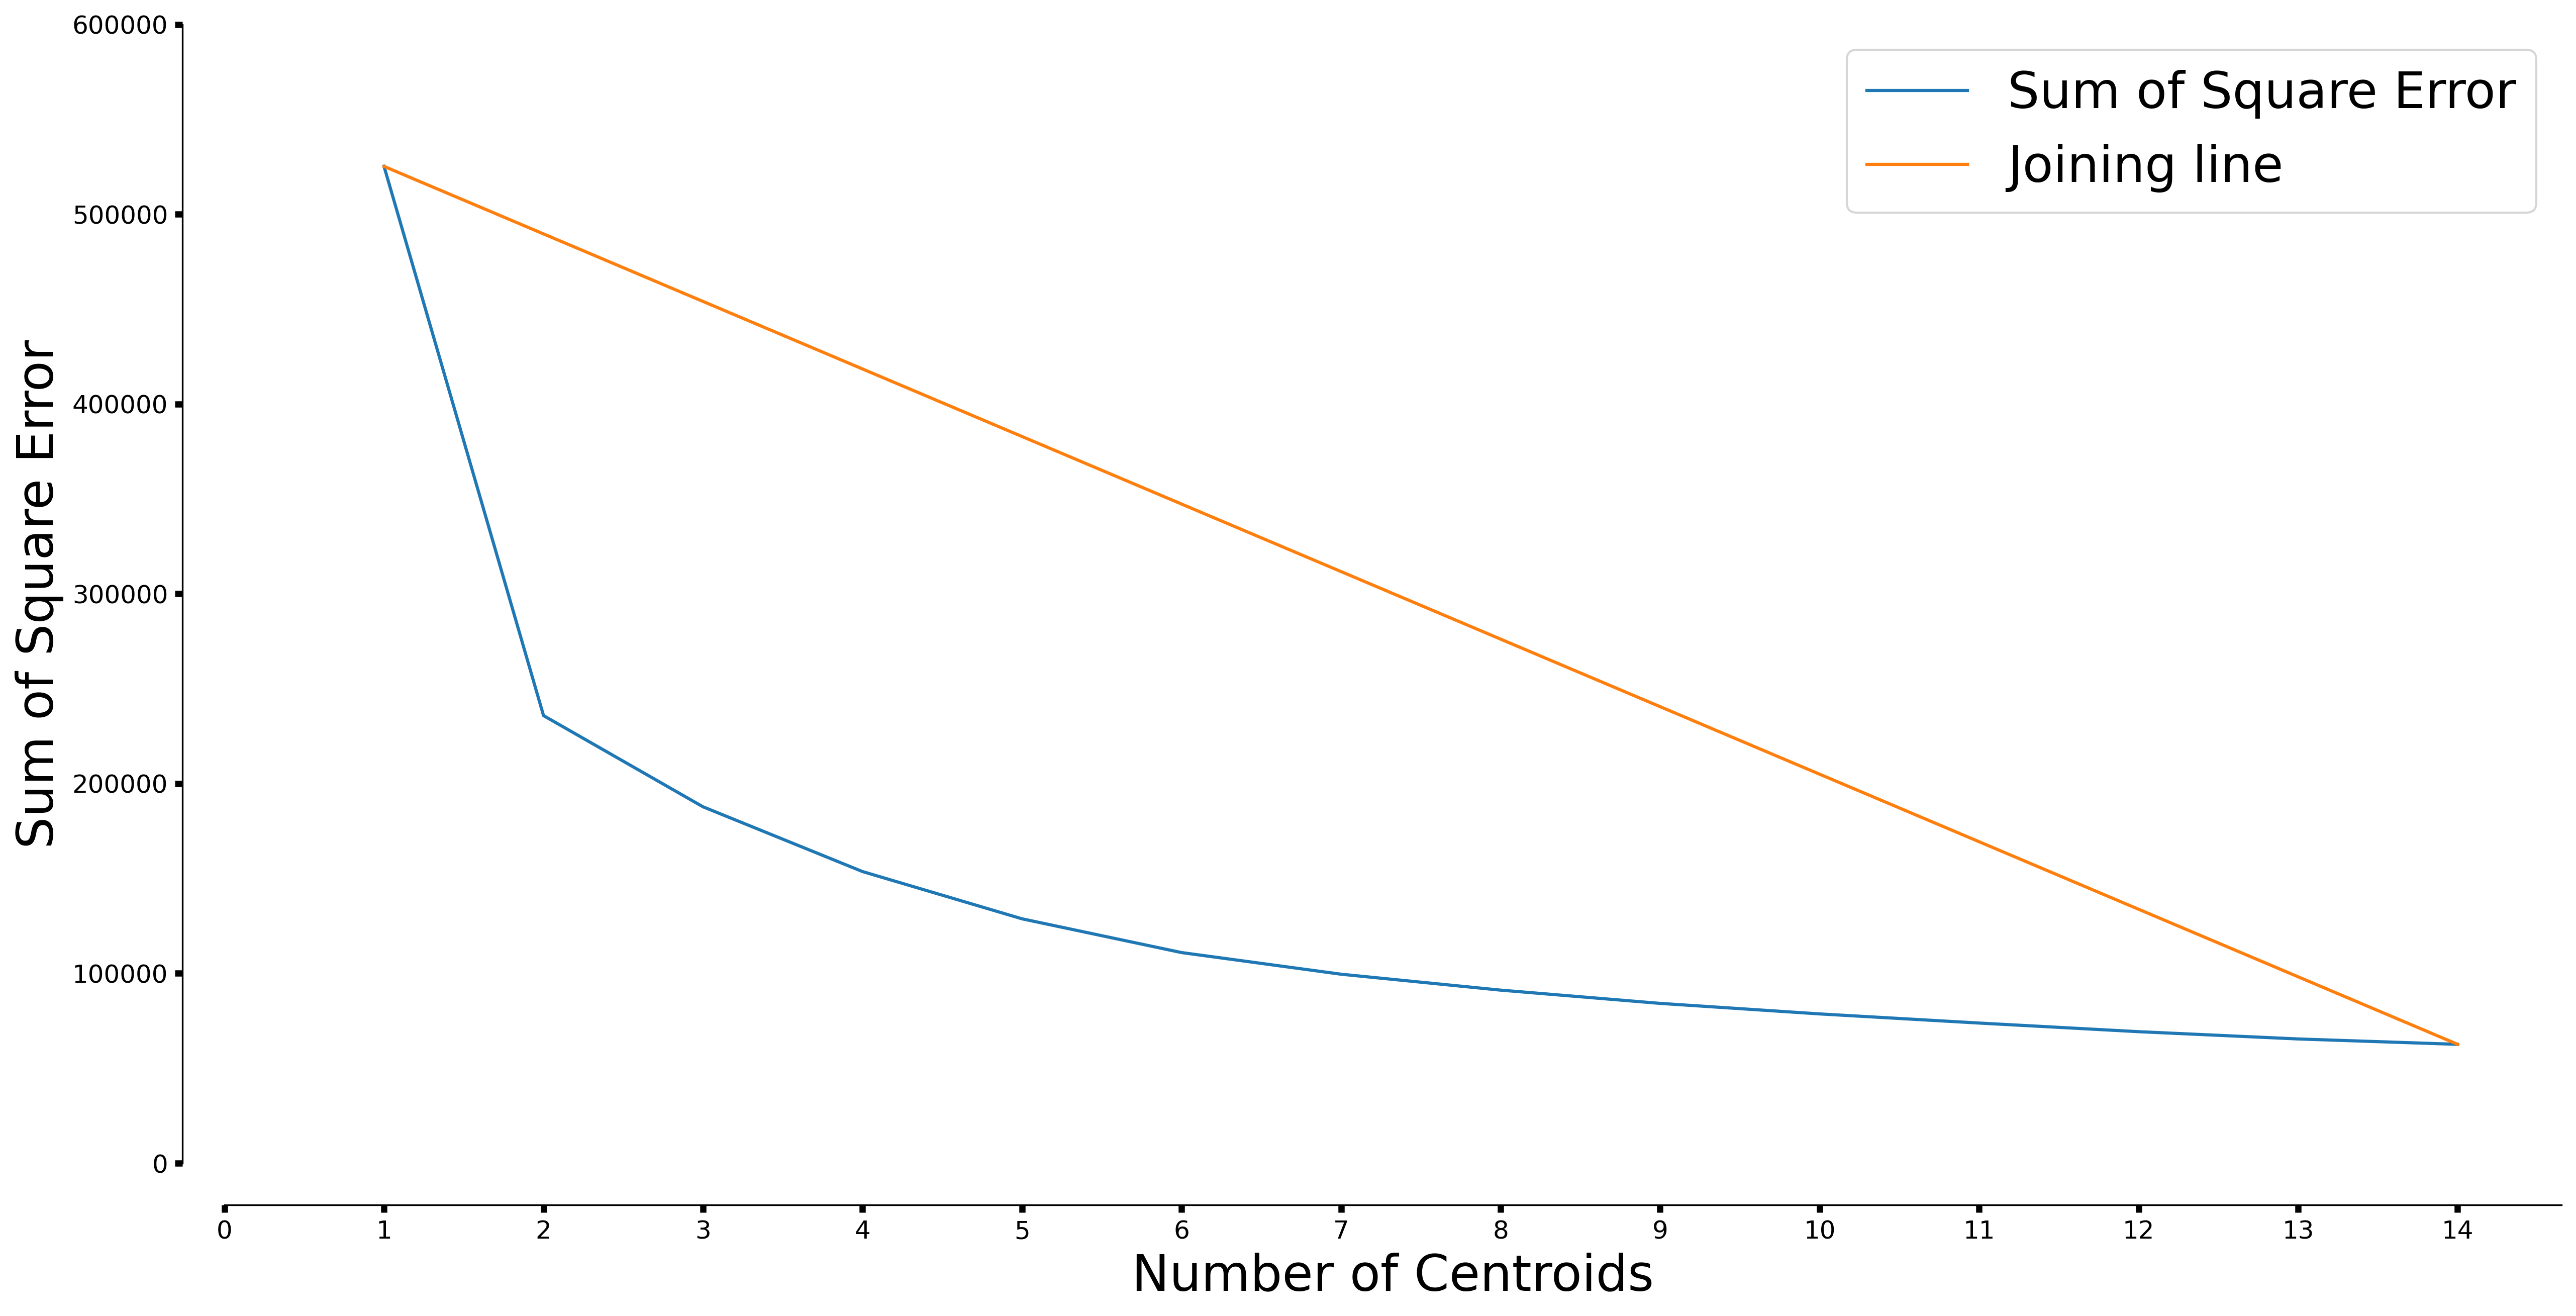
\includegraphics[scale=.3]{ElbowCurve.png}
		\caption{Intra-cluster variance vs the number fo clusters(blue); right joining firts and last point(orange). We can se the elbow shape of the graph; the elbow location in the one which maximize the distance between the right joining line and the elbow curve.}\label{fig:ElbowCurve}
	\end{figure}

	The optimal number of cluster is the one that corresponds to the elbow of the curve. It is difficult to find this feature from visually, I took the numerical value of the elbow considering the point which maximize the distance between the right joining the first and the last point.
	From this analysis I have found that the optimal number of clusters is $5$, which corresponds to the same that I have found considering the lung anatomy.
	
\end{document}